\chapter{Manual del usuario}

\section{Visión general}

\subsection{Introducción}

En el siguiente documento se recoge una descripción del funcionamiento del simulador de escenarios con usuarios móviles para la evaluación de algoritmos de recomendaciones.

\subsection{¿Que es el simulador de escenarios con usuarios móviles?}

El simulador de escenarios con usuarios móviles es una herramienta que trata de simular distintos tipos de algoritmos de recomendaciones en el entorno de una ciudad real con el fin de evaluar su correcto funcionamiento.

Se trata de un sistema multiusuario donde distintos tipos de usuarios se conectan y se mueven en una ciudad real (el entorno es configurado de antelación). El recomendador tiene en cuenta distintos tipos de parámetros: desde sus posiciones geográficas hasta sus perfiles y preferencias.

\subsection{Tipos de tecnologías utilizadas}

Esta herramienta consta de dos partes: la primera es el simulador y la segunda es el recomendador.

El Simulador esta desarrollado con nodejs, sockets-io, angularjs, bootstrap y como base de datos utiliza mongodb. El recomendador está desarrollado con java. La integración entre el navegador (cliente), simulador y recomendador está realizada mediante un sistema de evetos bidireccionales (sockets-io). De esta forma conseguimos comunicar todas la partes del sistema en tiempo real.

\subsection{Instalación}

\subsubsection{Paso 1: Instalar mongoDB}

Lo primero que tenemos que hacer es instalar mongodb. Los pasos para la instalación de mongodb depeden del tipo de sistema operativo que disponemos. Por esto no vamos a entrar en detalle de como se instala y vamos a seguir el tutorial disponible en la web oficial:

\begin{itemize}
	\item Linux: https://docs.mongodb.org/manual/administration/install-on-linux/
	\item Windows: https://docs.mongodb.org/manual/tutorial/install-mongodb-on-windows/
	\item Mac OS: https://docs.mongodb.org/manual/tutorial/install-mongodb-on-os-x/
\end{itemize}

\subsubsection{Paso 2: Instalar Node.js y NPM}

Vamos en la web oficial de nodejs (https://nodejs.org) y descargamos e instalamos la version v0.12.4. En el caso de Windows la instalación es igual que la de cualquier otro programa. Para la instalación en otros SO visitar https://nodejs.org/en/download/.

A continuación tenemos que instalar el gestor de paquetes NPM v2.10.1. En el caso de Windows vamos en la web oficial (https://nodejs.org/en/download/) y nos descargamos e instalamos el ejecutable. En el caso de Linux ejecutamos el siguiente comando en la consola:
\begin{lstlisting}[language=xml, frame=single]
sudo apt-get install npm
\end{lstlisting}

\subsubsection{Paso 3: Instalar git}

Git es un sistema distribuido de control de versiones. Para la instalación de este nos descargamos el ejecutable de https://git-scm.com/downloads y seguimos los pasos que nos indica este.

\subsubsection{Paso 4: Clonar el proyecto de github e instalarlo}

A continuacion tenemos que clonar el proyecto del Simulador de github. Para esto abrimos una consola y nos situamos en el directorio donde queremos clonar el proyecto. A continuacion ejecutamos el siguiente comando:
\begin{lstlisting}[language=xml, frame=single]
git clone https://github.com/slavcho87/Simulator
\end{lstlisting}
Vemos que se ha creado un directorio llamado Simulator. Lo primero que tenemos que hacer es bajarnos todas las dependencias del proyecto. Por esto ejecutamos el siguiente comando:
\begin{lstlisting}[language=xml, frame=single]
npm install
\end{lstlisting}
Una vez que nos hemos clonado el proyecto y descargado las dependencias de este podemos arrancar el servidor mediante el siguiente comando:
\begin{lstlisting}[language=xml, frame=single]
npm start
\end{lstlisting}

\paragraph{Paso 4.1: Configuraciones básicas del simulador}

En el fichero baseConfig.json disponemos de las siguientes basicas para el simulador como el puerto donde se ejecuta el servidor y la localizacion de la base de datos. Si editamos el fichero baseConfig.json veremos que tiene el siguiente contenido:
\begin{lstlisting}[language=xml, frame=single]
{ 
"port": 81, 
"locationDB": "localhost", 
"nameDB": "simulator" 
}
\end{lstlisting}

Las variables del fichero baseConfig.json tienen el siguiente significado:

\begin{itemize}
	\item port: es el puerto donde se va a ejecutar el servidor
	\item locationDB: es la localizacion donde se va a ejecutar mongodb.
	\item nameDB: es el nombre del esquema de la base de datos donde nos conectamos.
\end{itemize}

Dichas configuraciones son importantes ya que de esta forma tenemos la opción de llevarnos la base de datos en un servidor diferente para darle más potencia.

\subsubsection{Paso 5: Instalación del recomendador}

\paragraph{Paso 5.1: Instalar Apache maven}

Antes de todo tenemos que instalar Apache maven que es un gestor de paquetes. Por lo tanto vamos en la web oficial (https://maven.apache.org/) y descargamos y descomprimimos el ficheros compromido. A continuación tenemos que añadir en la variable PATH la dirección de la carpeta donde hemos descomprimido maven. Para ver que maven se haya instalado correctamente ejecutamos el siguiente comando:
\begin{lstlisting}[language=xml, frame=single]
mvn -v
\end{lstlisting}
De esta forma comprobamos la version de maven que tenemos instalado. Tenemos que ver una salida como la siguiente: \newline

\begin{lstlisting}[language=xml, frame=single]
Apache Maven 3.2.5 (12a6b3acb947671f09b81f49094c53f426d8cea1; 2014-12-14T18:29:23+01:00)
Maven home: C:\maven
Java version: 1.7.0_79, vendor: Oracle Corporation
Java home: C:\Program Files (x86)\Java\jdk1.7.0_79\jre
Default locale: es_ES, platform encoding: Cp1252
OS name: "windows 8.1", version: "6.3", arch: "x86", family: "windows"
\end{lstlisting}

\paragraph{Paso 5.2: Compilar el recomendador}

Una vez que hayamos instalado maven correctamente tenemos que compilar el recomendador. Por esto ejecutamos el ficheros compilarRecommender que se encuentra en la carpeta scripts. Existen dos versiones: uno para Windows y otro para Linux.

\paragraph{Paso 5.3: Configuraciones básicas del recomendador}

Si editamos el fichero configs/baseConfig.txt podemos ver que tiene el siguiente formato:
\begin{lstlisting}[language=xml, frame=single]
<config>
<host>http://localhost</host>
<port>81</port> 
<hostMongo>localhost</hostMongo>
<portMongo>27017</portMongo> 
<nameDB>simulator</nameDB> 
</config>
\end{lstlisting}

\begin{itemize}
	\item host: es la dirección donde se ejecuta el simulador. En el ejemplo este se está ejecutando en local
	\item port: es el puerto donde se ejecuta el simulador. En el ejemplo este se ejecuta en el puerto 81
	\item hostMongo: es la dirección de la base de datos. En el ejemplo esta se está ejecutando en local
	\item portMongo: es el puerto donde se ejecuta la base de datos.
	\item nameDB: es el nombre del esquema de la base de datos
\end{itemize}

\paragraph{Paso 5.4: Ejecutar el recomendador}

Para ejecutar el recomendar tenemos que ejecutar el ficheros ejecutarRecommender que se encuentra en la carpeta scripts. Existe dos versiones de este fichero: uno para Windows y otro para Linux.

\subsection{Primeros pasos}

El primero paso al instalar el simulador es crear nuestro usuario (apartado \ref{sec:CrearUsuario}). A continuación vamos en Settings y realizamos las configuraciones realizadas en los capítulos \ref{sec:confRecomendador}, \ref{sec:confObjEstaticos} y \ref*{sec:confObjDinamicos}.

Se trata de crear nuevas configuraciones para el recomendador y crear los tipos de objetos dinámicos y estáticos que usaremos posteriormente en la creación de mapa (apartado \ref{sec:crearMapa}) y escenas (apartado \ref{sec:crearEscena}).

\section{Configuración del recomendador}\label{sec:confRecomendador}

Para configurar los parámetros del recomendador primero tenemos que estar autentificados con nuestros usuario. Una vez autentificados vamos en Settings $\rightarrow$ Recommender settings y vemos la siguiente pantalla:

\begin{figure}[H]
	\centering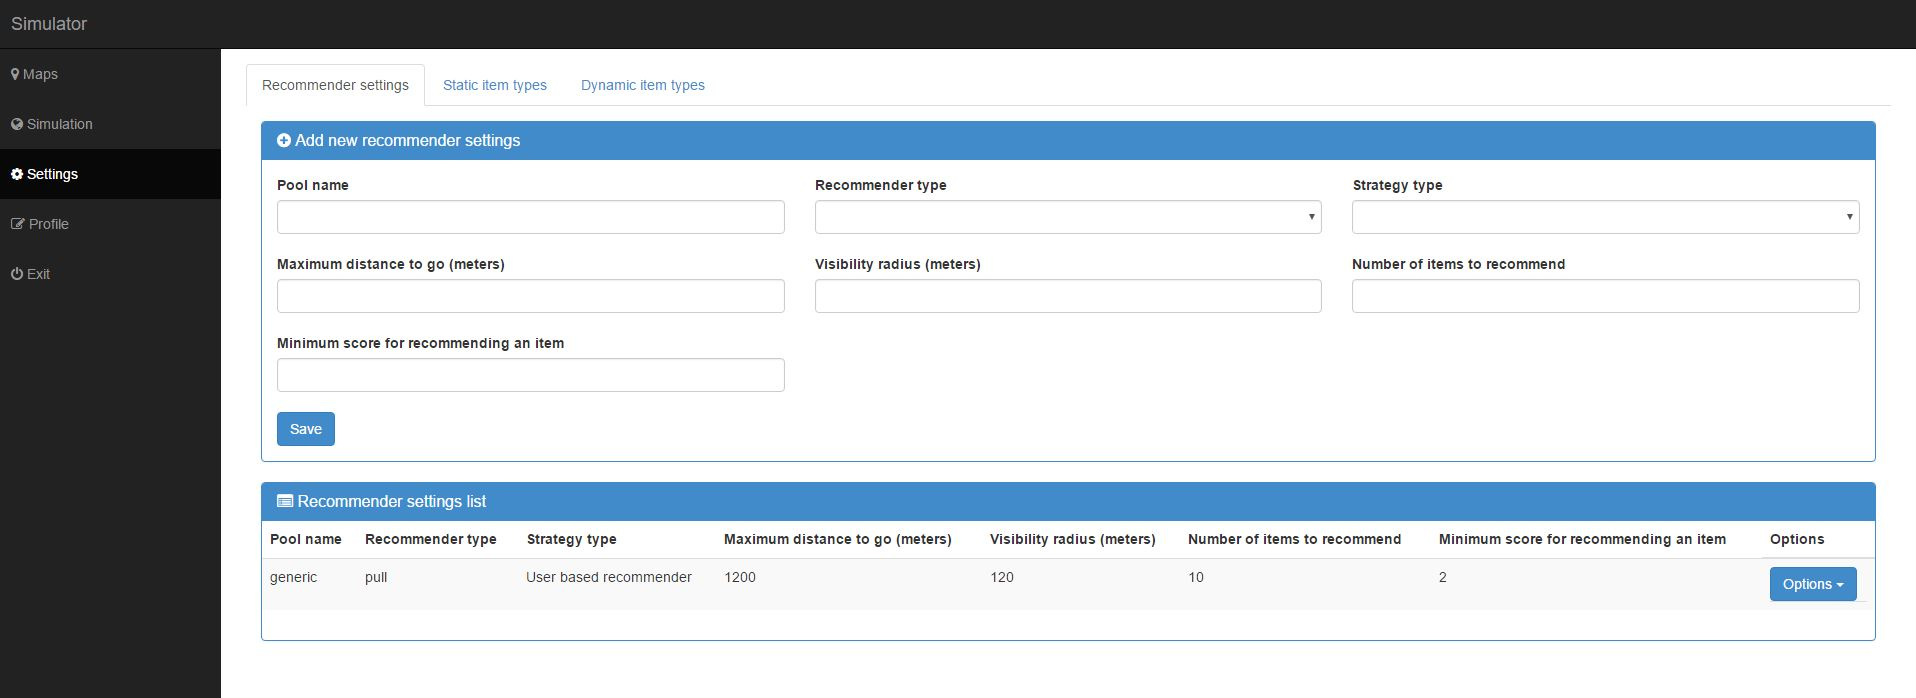
\includegraphics[scale=0.3]{imagenes/capitulo2/configuracion-recomendador.jpg}
	\caption{Configuración del recomendador}
	\label{img:ConfiguracionRecomendador}
\end{figure}

\newpage

En este formulario tenemos que introducir los siguientes datos:
\begin{itemize}
	\item Pool name: es nombre que vamos a dato al conjunto de parámetros
	\item Recommender type: es el tipo de recomendador. Podemos elegir entre pull (el usuario solicita una recomendación) o push (el recomendador realiza recomendaciones sin que el usuario lo haya solicitado)
	\item Strategy type:: indicar el tipo de implementación que queremos para el recomendador
	\item Maximum distance to go (meters): es la distancia máxima (en metros) que está dispuesto a recorrer el usuario
	\item Visibility radius (meters): radio (en metros) de visibilidad del usuario. Los items que están fuera de este radio son invisibles para el usuario 
	\item Number of items to recommend: número máximo de items que va a recomendar el recomendador cada vez
	\item Minimum score for recommending an item: puntuación mínima para que un item sea recomendado
\end{itemize}

\section{Configuración de los objetos estáticos}\label{sec:confObjEstaticos}

Para crear un nuevo tipo de objeto estático primero tenemos que estar autentificados con nuestros usuario. Una vez autentificados vamos en Settings $\rightarrow$ Static item type y vemos la siguiente pantalla:

\begin{figure}[H]
	\centering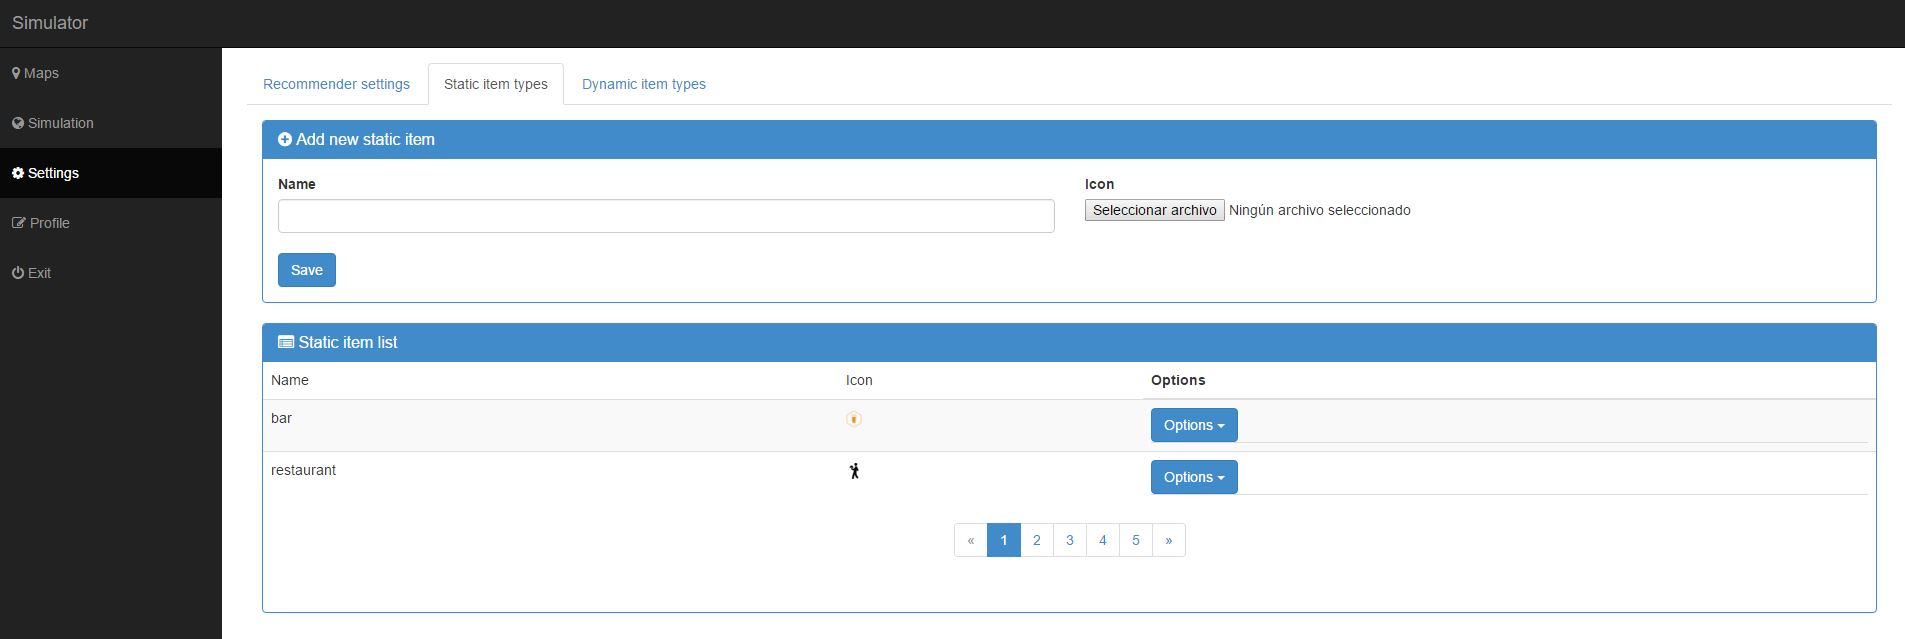
\includegraphics[scale=0.3]{imagenes/capitulo3/config-objetos-estaticos.jpg}
	\caption{Configuración de los objetos estáticos}
	\label{img:ConfiguracionObjetosEstaticos}
\end{figure}

\newpage

En este formulario tenemos que introducir los siguientes datos:

\begin{itemize}
	\item Name: es el nombre del tipo del objeto estático
	\item Icon: icono del tipo del objeto estático
\end{itemize}	

Por debajo del formulario de creación nuevos tipos de objetos estáticos aparecerá la lista con todos los tipos de objetos estáticos que han sido creados. En el apartado opciones podemos gestionar cada uno de estos objeto.

\section{Configuración de los objetos dinámicos}\label{sec:confObjDinamicos}

Para crear un nuevo tipo de objeto dinámicos primero tenemos que estar autentificados con nuestros usuario. Una vez autentificados vamos en Settings $\rightarrow$ Dynamic item type y vemos la siguiente pantalla:

\begin{figure}[H]
	\centering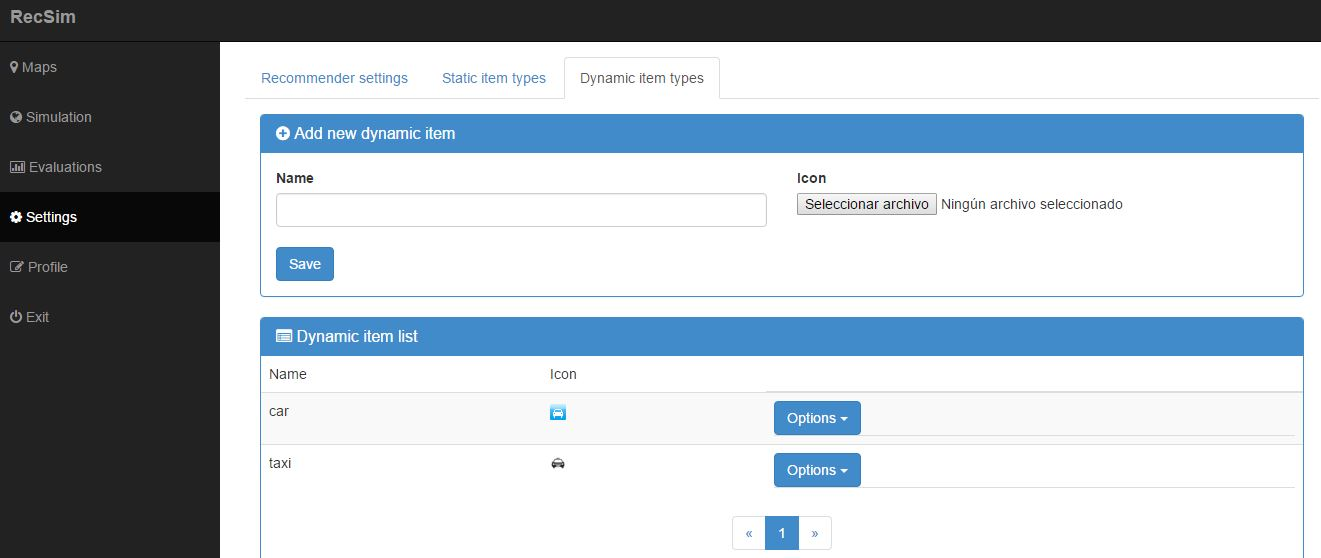
\includegraphics[scale=0.3]{imagenes/capitulo4/config-objetos-dinamicos.jpg}
	\caption{Configuración del recomendador}
	\label{img:ConfiguracionObjetosDinamicos}
\end{figure}

En este formulario tenemos que introducir los siguientes datos:

\begin{itemize}
	\item Name: es el nombre del tipo del objeto dinámicos
	\item Icon: icono del tipo del objeto dinámicos
\end{itemize}

Por debajo del formulario de creación nuevos tipos de objetos dinámicos aparecerá la lista con todos los tipos de objetos dinámicos que han sido creados. En el apartado opciones podemos gestionar cada uno de estos objeto.

\section{Crear un un nuevo usuario}\label{sec:CrearUsuario}

Para registrar un nuevo usuario lo que tenemos que hacer es pinchar en el enlace Register en la página lo login. Se nos muestra la siguiente pantalla:

\begin{figure}[H]
	\centering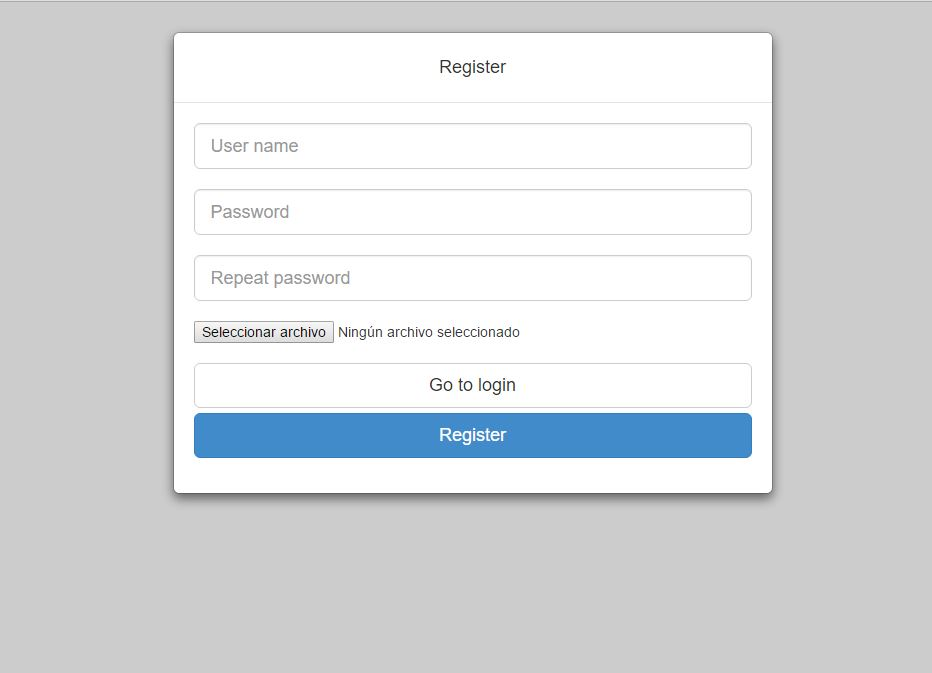
\includegraphics[scale=0.3]{imagenes/capitulo5/register.jpg}
	\caption{Crear un nuevo usuario}
	\label{img:AddUser}
\end{figure}

En este formulario tenemos que añadir el nombre del usuario, su contraseña y subir su imagen. Esta imagen aparecerá en el mapa del simulador. Una vez que hayamos creado el usuario tenemos que pulsar el botón "Go to login" para volver en la pantalla de login para introducir el nombre de nuestro usuario su contraseña.

\section{Actualizar el perfil de un usuario}

Para realizar cambios en el nombre del usuario, cambiar la imagen del perfil o cambiar la contraseña tenemos que ir en el menú Perfil:

\begin{figure}[H]
	\centering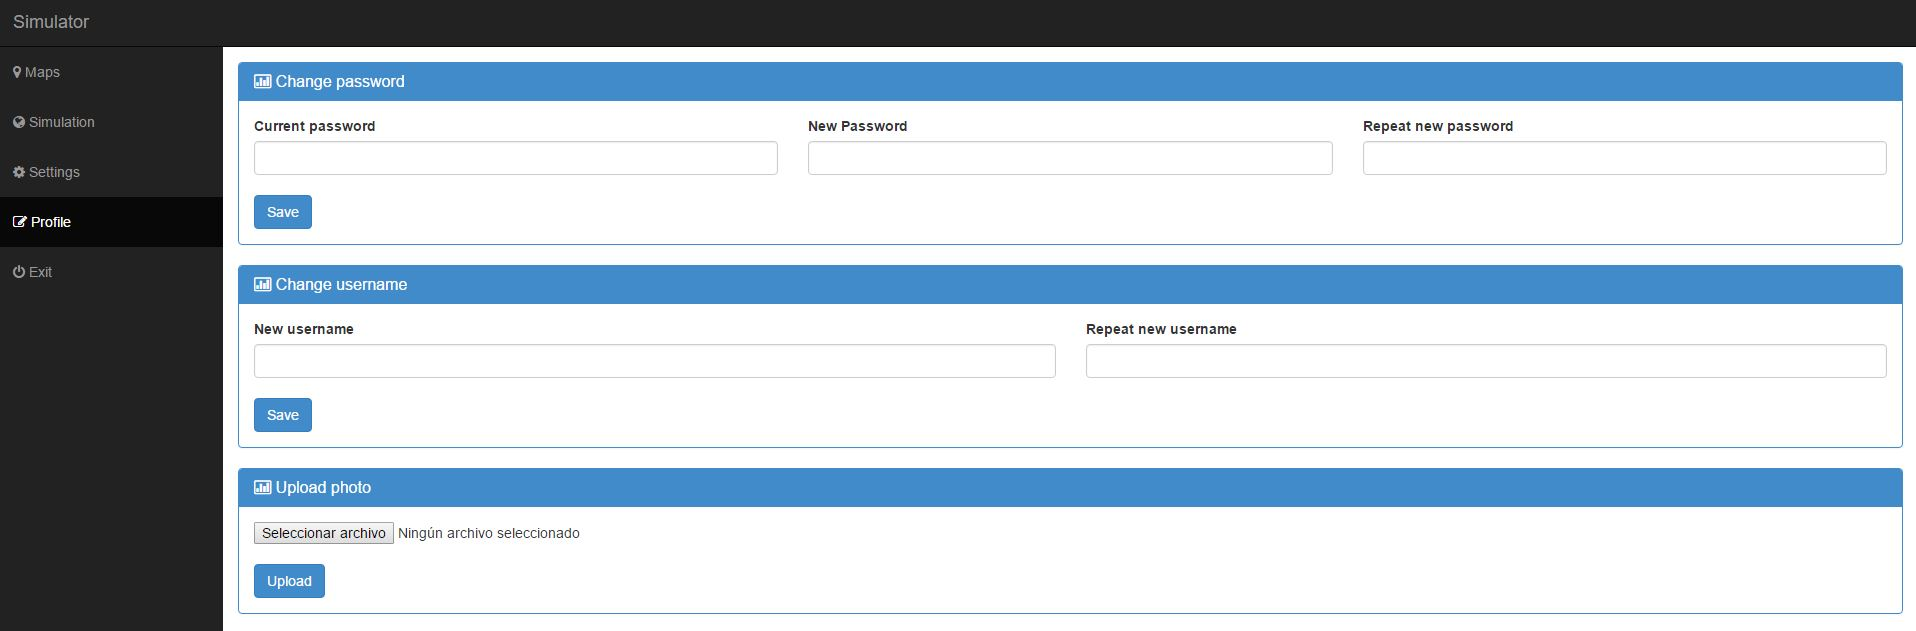
\includegraphics[scale=0.3]{imagenes/capitulo6/perfil-del-usuario.jpg}
	\caption{Actualizar el perfil de un usuario}
	\label{img:UpdateUser}
\end{figure}

Vemos que hay 3 formularios:

\begin{itemize}
	\item uno para cambiar el nombre del usuario
	\item otro para cambiar la contraseña del usuario
	\item otro para cambiar la imagen del perfil del usuarios
\end{itemize}

Al realizar cualquier cambio el el sistema nos informara si la acción ha salido bien o no.

\section{Búsqueda de mapas}\label{sec:BuscarMapas}

La opción Maps $\rightarrow$ map search nos permite buscar mapas a los cuales queremos conectarnos para realizar alguna simulación:

\begin{figure}[H]
	\centering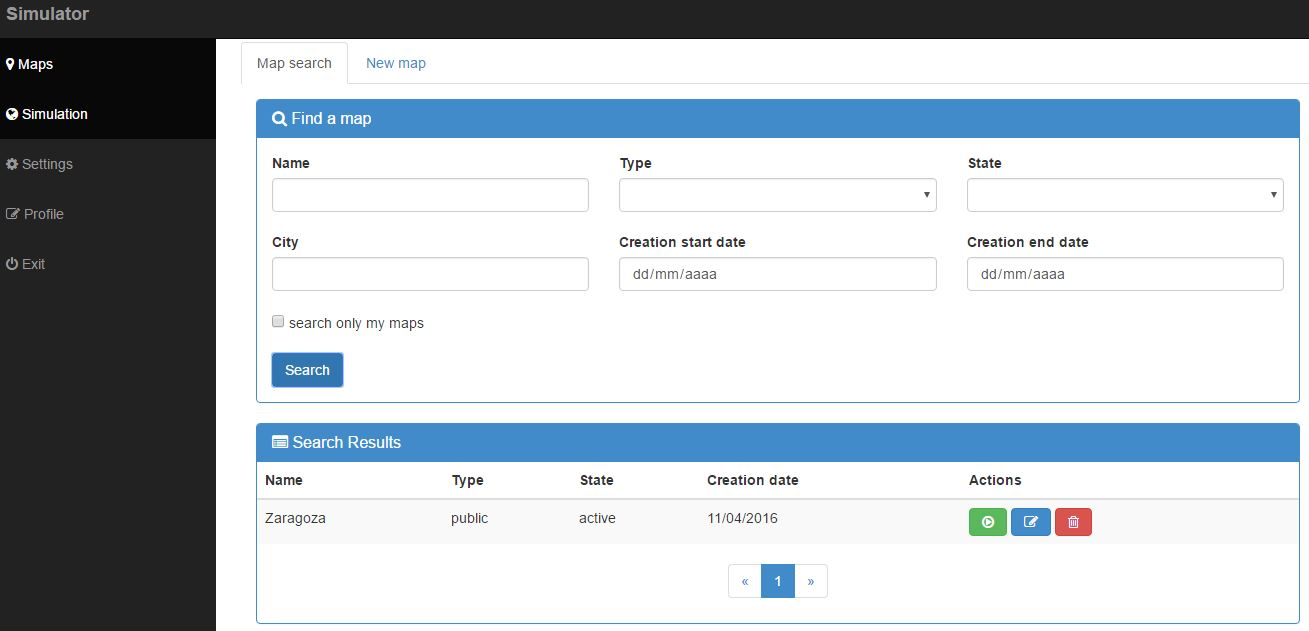
\includegraphics[scale=0.3]{imagenes/capitulo7/busqueda-de-mapas.jpg}
	\caption{Búsqueda de mapas}
	\label{img:BuscarMapas}
\end{figure}

En la imagen vemos que disponemos de distintos tipos de filtros para la búsqueda de mapas. Estos filtros son: por nombre, por tipo, por estado, por ciudad, por fechas de creación o solo buscar solo mis mapas. Si no introducimos ningún filtro devolverá todos los mapas que están creados en el sistema.

\newpage

\section{Crear un nuevo mapa}\label{sec:crearMapa}

Para crear un nuevo mapa vamos en Maps $\rightarrow$ new map y vemos el siguiente formulario:

\begin{figure}[H]
	\centering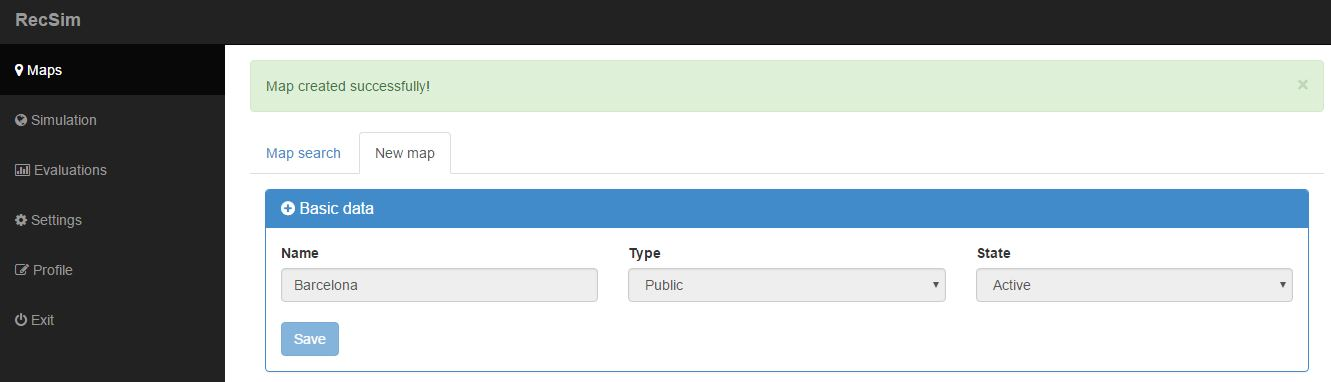
\includegraphics[scale=0.3]{imagenes/capitulo8/crear-un-nuevo-mapa.jpg}
	\caption{Crear un nuevo mapa}
	\label{img:AddMapa}
\end{figure}

Tenemos que rellenar los siguientes datos:

\begin{itemize}
	\item Name: es el nombre que queremos dar al mapa.
	\item Type: tipo que mapa. Podemos elegir entre publico (puede conectarse cualquier usuarios) y privado (solo puede conectarse el que la ha creado).
	\item State: estado del mapa. Podemos elegir entre activa (que el mapa está disponible para realizar simulaciones) y borrador (el mapa todavía no está disponible para realizar simulaciones)
\end{itemize}

Una vez que hayamos rellenado el formulario pulsamos en el botón Save y el sistema nos informara si el guardado ha salido con éxito o no. Si se ha guardado con éxito por debajo de este formulario aparece el formulario de creaciones de escenas y una lista de las escenas actuales. Lo normales es que la lista de escenas creadas aparezca vacía ya que todavía no hemos creado ninguna escena. Para ver los detalles de como crear una escena consultar el capítulo \ref{sec:crearEscena}.

\section{Crear una nueva escena}\label{sec:crearEscena}

Una vez que hayamos creado el mapa podemos empezar a crear las escenas. La creación de escenas se realiza en 4 pasos. En el primero de los pasos tenemos que introducir el nombre de la escenas y el elegir el tipo de recomendador que queremos usar para dicha escena:

\begin{figure}[H]
	\centering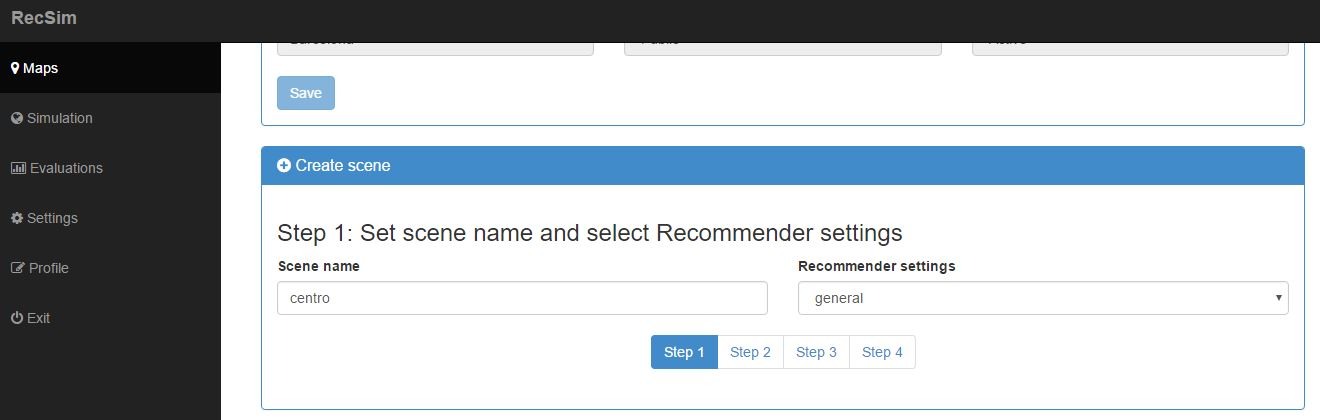
\includegraphics[scale=0.3]{imagenes/capitulo9/crear-escena-1.jpg}
	\caption{Crear una nueva scena}
	\label{img:AddScena1}
\end{figure}

En el segundo paso tenemos que elegir en que cuidad se va a realizar la simulación y definir los limites de la escena:

\begin{figure}[H]
	\centering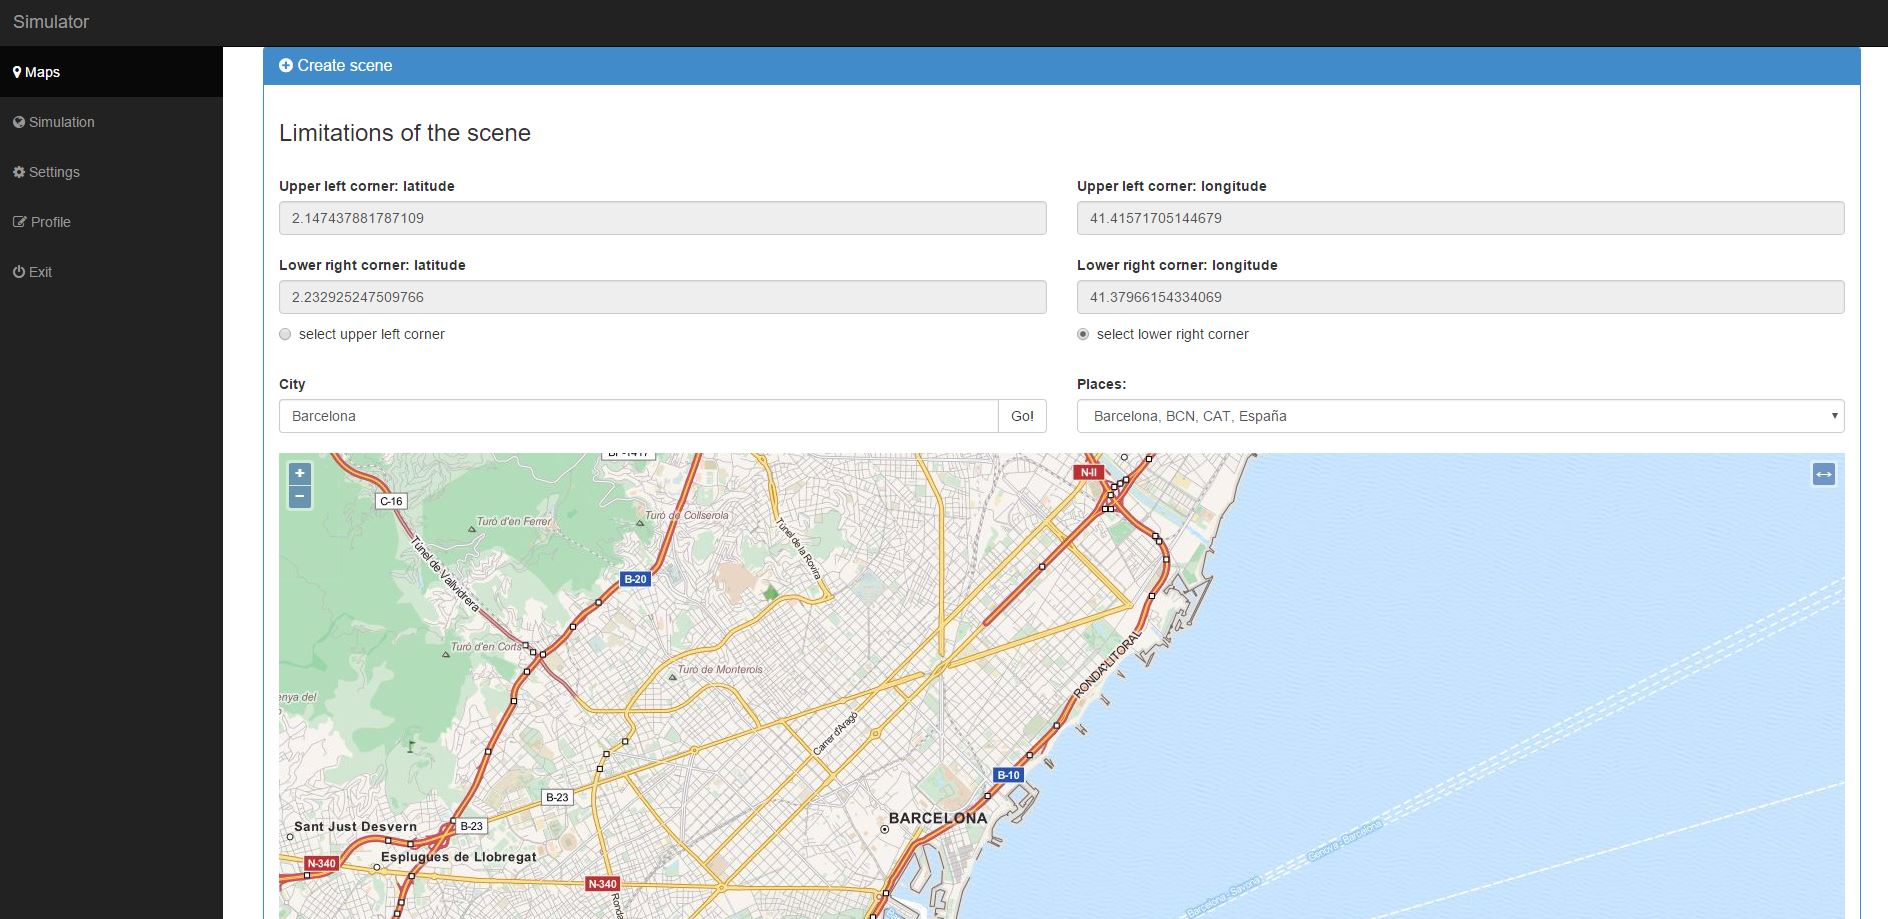
\includegraphics[scale=0.3]{imagenes/capitulo9/crear-escena-2.jpg}
	\caption{Crear una nueva scena}
	\label{img:AddScena2}
\end{figure}

Para definir los limites de la escena tenemos que definir las dos esquinas (superior izquierda e inferior derecha). Por lo tanto para definir la esquina superior izquierda seleccionamos la opción select upper left corner y hacemos click en el mapa para definir donde estará dicha esquina. Veremos que las cajas de texto Upper left corner: latitude y Upper left corner: longitude aparecerán las coordenadas geográficas de dicha esquina (longitud y latitud).

Para definir la esquina inferior derecha seleccionamos la opción select lower right corner y hacemos click en el mapa para definir donde estará dicha esquina. Cuando hayamos seleccionado la esquina inferior derecha vemos que en las cajas de texto Lower right corner: latitude y Lower right corner: longitude aparecerán las coordenadas geográficas de dicha escena.

En el tercer paso tenemos que definir los objetos estáticos de la escena:

\begin{figure}[H]
	\centering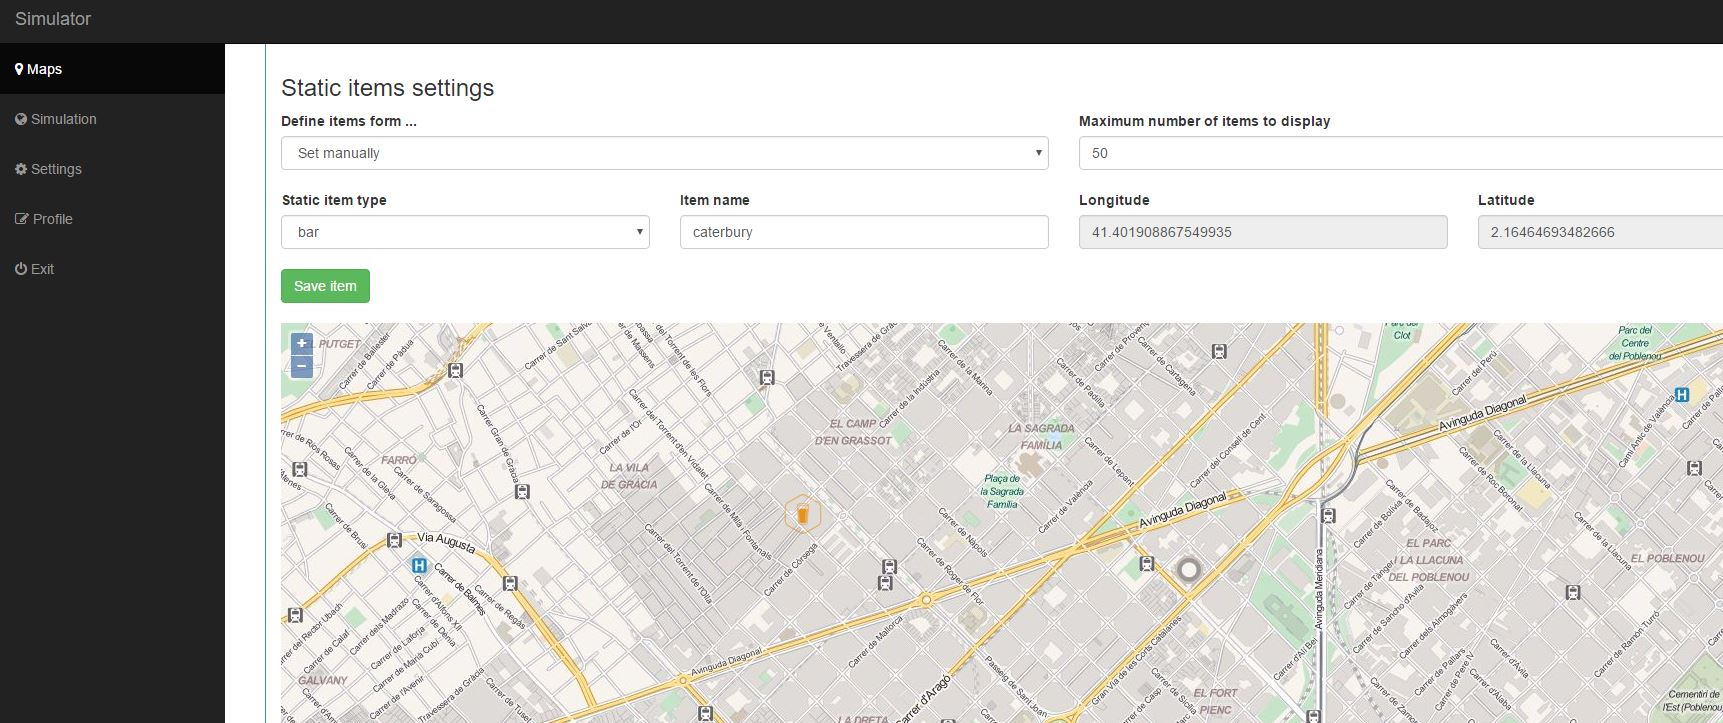
\includegraphics[scale=0.3]{imagenes/capitulo9/crear-escena-3-1.jpg}
	\caption{Crear una nueva scena}
	\label{img:AddScena31}
\end{figure}

Hay dos maneras para definir objetos estáticos: manualmente y importándolos desde un fichero. Para definirlos de forma manual tenemos que elegir la opción set manually y aparecerá un formulario en el cual tenemos que elegir el tipo de objeto estático, introducir su nombre y seleccionar en el mapa donde queremos situarlo. Una vez que hayamos introducir estos datos tenemos que pulsar el botón Save item para confirmar que queremos que dicho objeto forme parte de la escena.

Por debajo del mapa podemos ver una lista con todos los objetos estáticos de la escena y una opción que nos permite borrar los objetos que no necesitamos:

\begin{figure}[H]
	\centering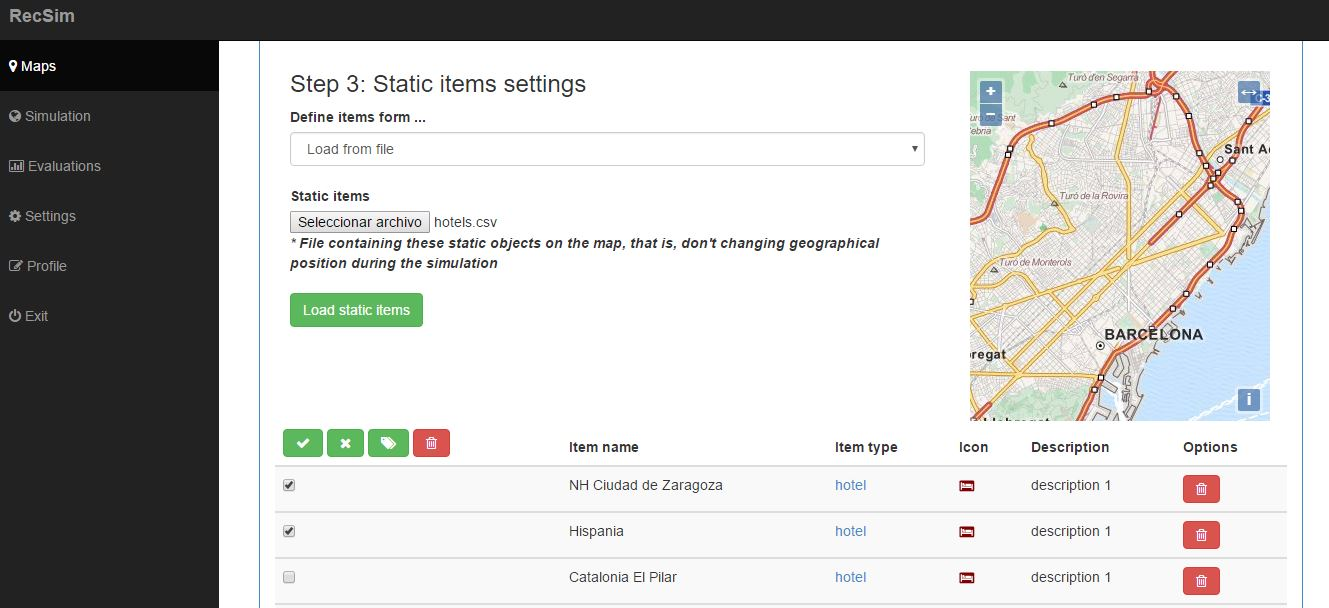
\includegraphics[scale=0.3]{imagenes/capitulo9/crear-escena-3-2.jpg}
	\caption{Crear una nueva scena}
	\label{img:AddScena32}
\end{figure}

En el cuarto y último paso tenemos que definir cuales son los objetos dinámicos y sus rutas:

\begin{figure}[H]
	\centering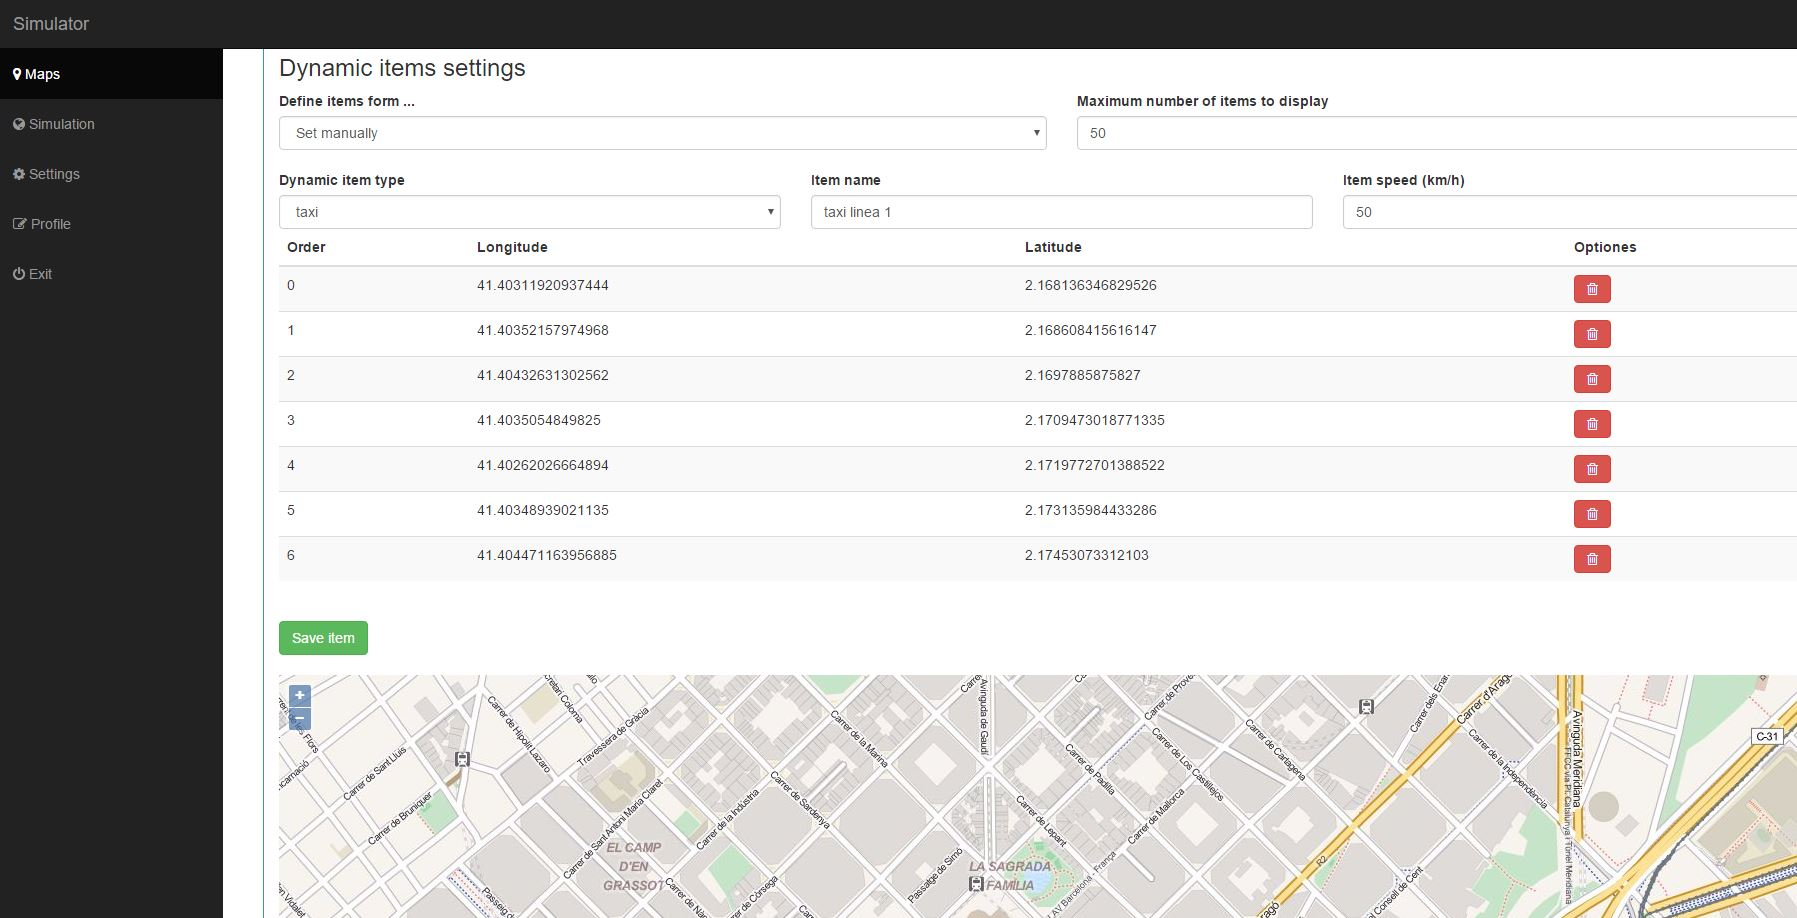
\includegraphics[scale=0.3]{imagenes/capitulo9/crear-escena-4.jpg}
	\caption{Crear una nueva scena}
	\label{img:AddScena4}
\end{figure}

Igual que los objetos estáticos también tenemos dos formas de definir los objetos dinámicos: manual e importando un fichero. La forma manual consiste en elegir que tipo de objeto dinámico queremos introducir, su nombre, velocidad y ruta. Para introducir la ruta es suficiente con ir seleccionando sobre el mapa los nodos de movimiento del objeto. Al final pulsamos sobre el botón Save item para confirmar que queremos que este objeto forme parte de la escena. Una vez confirmado esto por debajo del mapa vemos una lista con todos los objetos dinámicos introducidos hasta el momento y podemos borrar alguno de ellos si es necesario:

\begin{figure}[H]
	\centering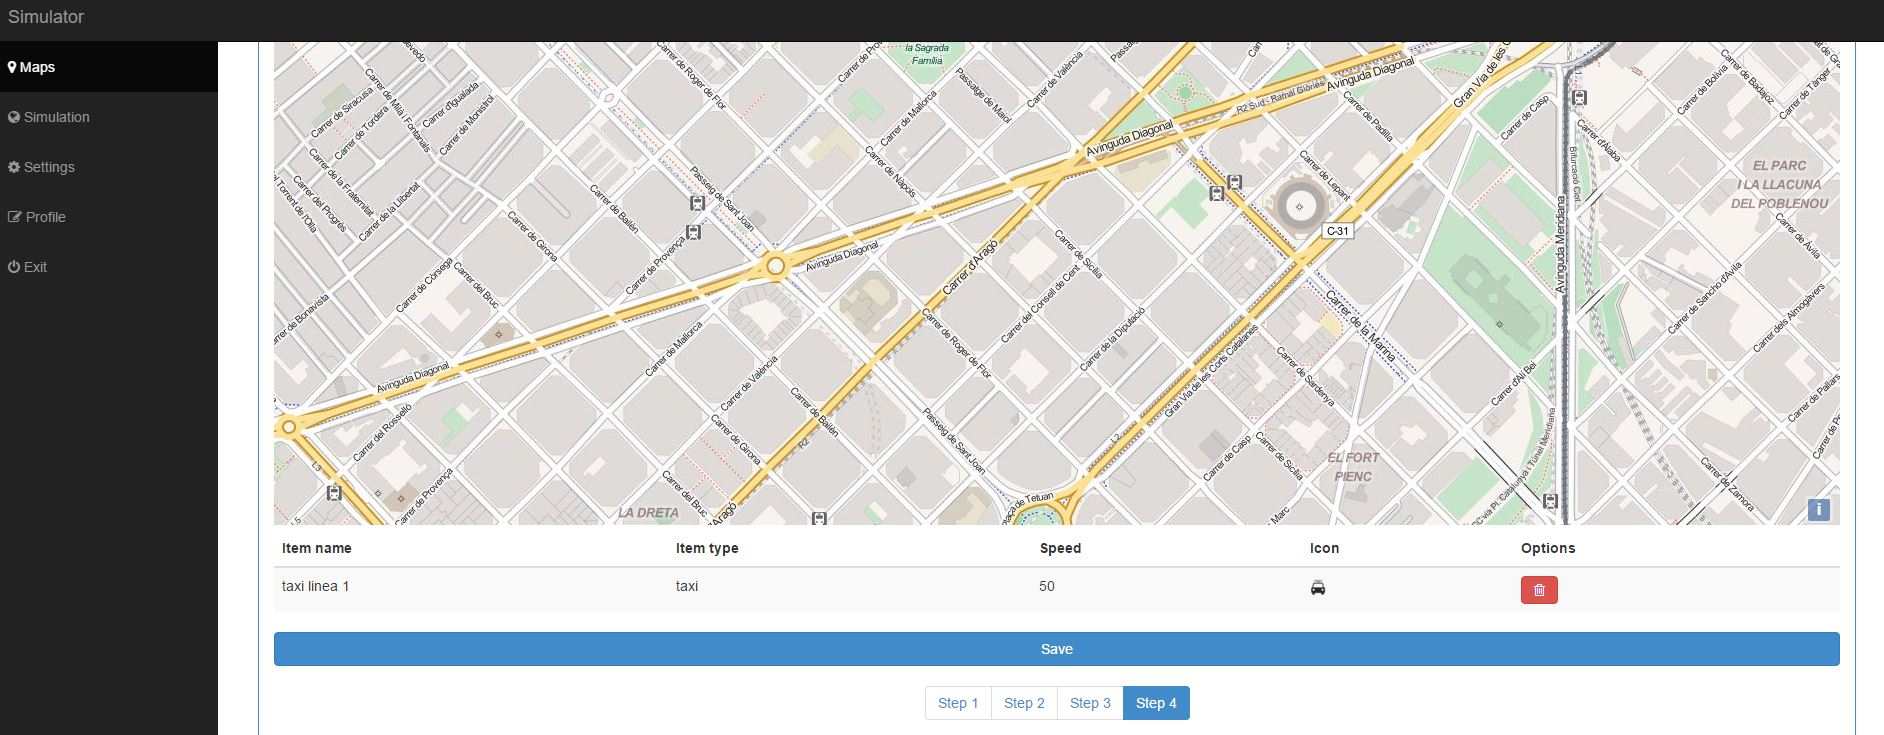
\includegraphics[scale=0.2]{imagenes/capitulo9/crear-escena-4-1.jpg}
	\caption{Crear una nueva scena}
	\label{img:AddScena41}
\end{figure}

Una vez introducidos todos los datos pulsamos el botón Save para crear la escena y cuando se haya creado por debajo aparece una lista con todos los escenarios creados hasta el momento donde podemos editar o borrar escenas. Si el mapa no tiene escenas asociadas es que la lista no aparezca.

\section{Edición de mapas y escenas}

Para modificar un mapa o escena primero tenemos que realizar una busque de mapas en Maps $\rightarrow$ maps search y en la lista de resultados pulsamos sobre el icono de editar imagen. Solo podemos editar un mapa si la hayamos creado nosotros. De lo contrario el icono de editar imagen no aparecerá. Una vez que hayamos pulsado el icono de editar imagen entonces veremos la siguiente pantalla:

\begin{figure}[H]
	\centering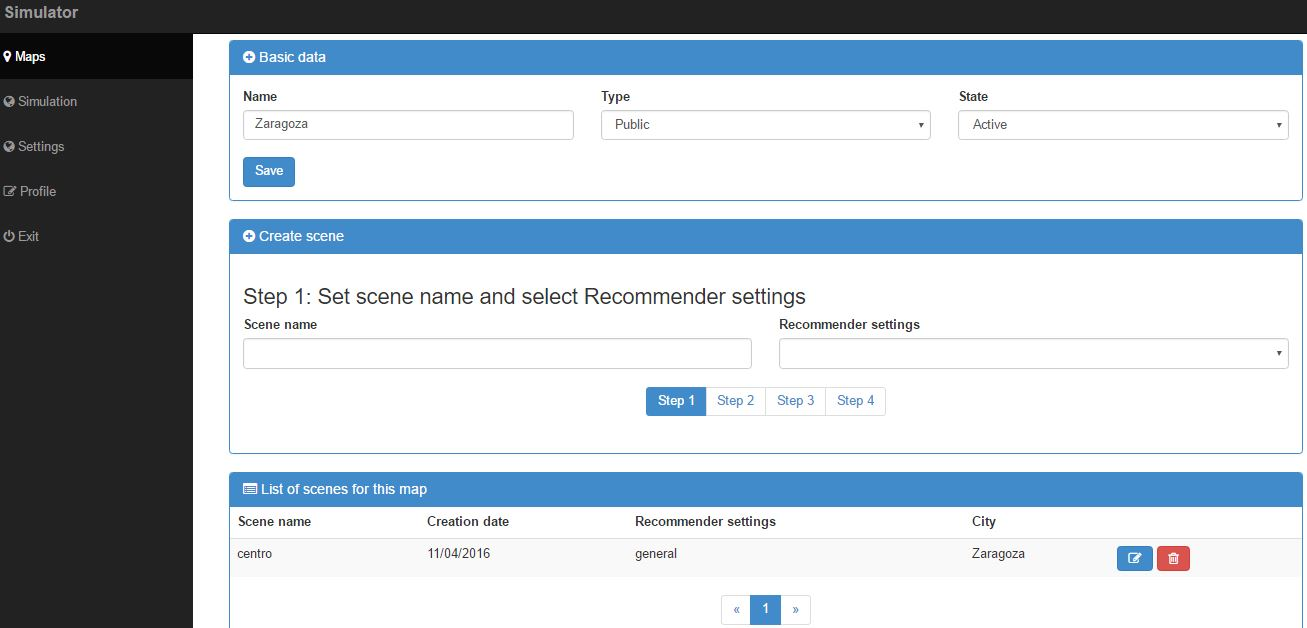
\includegraphics[scale=0.3]{imagenes/capitulo10/capitulo10.jpg}
	\caption{Edición de mapas y escenas}
	\label{img:UpdateMapScene}
\end{figure}

En esta pantalla disponemos de distintos tipos de opciones entre los cuales modificar datos del mapa, crear o modificar escenas.

\newpage

\section{Simulación}

Para ejecutar una simulación lo primero que tenemos que hacer es realizar la búsqueda de un mapa explicado en el capítulo \ref{sec:BuscarMapas}. Una vez que hayamos realizado la búsqueda pulsamos el botón "Play" y a continuación se nos muestra una pantalla en la cual tenemos que elegir la escena a la cual queremos conectarnos.

\begin{figure}[H]
	\centering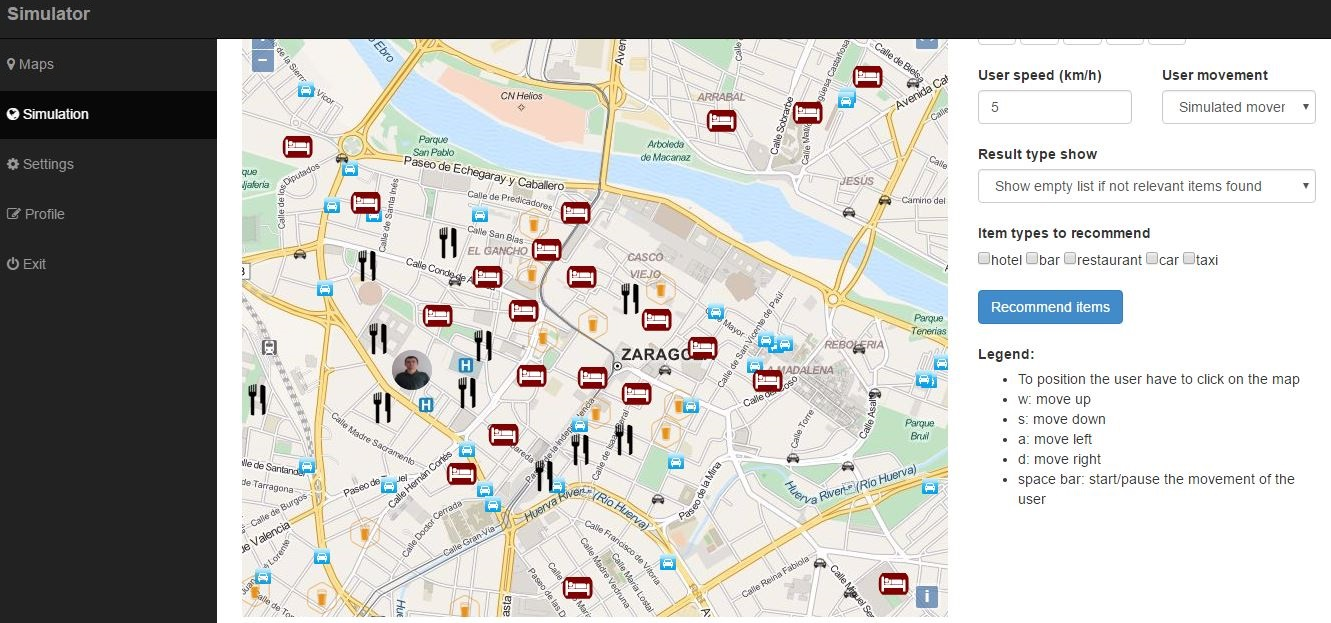
\includegraphics[scale=0.3]{imagenes/capitulo11/capitulo11.jpg}
	\caption{Simulación}
	\label{img:Simulation}
\end{figure}